%\fancyfoot[L]{$ $Date$ $}
%\fancyfoot[R]{$ $Revision$ $}

\chapter{Neoclassical background}

By default the background distribution function in considered to be a Maxwellian.  However due to background flows the temperature and density 
gradients, coupled with the geometry and collisions, the distribution function can deviate from the Maxwellian by a small amount.   This section describes the implementation of the interface between NEO and GKW so that small deviations from background Maxwellian can be included.

\section{Form of the equations for arbitrary background}

The corrections to the background Maxwellian are calculated, at the moment, by the Eulerian
Neoclassical transport code {\small NEO} \cite{NEO1,NEO2}.  

We start with the gyro-kinetic Vlasov equation in (${\bf X}, v_\parallel, 
\mu$) coordinates,
\begin{equation}
{\partial f_{\rm tot} \over \partial t} + {{\rm d} {\bf X} \over {\rm d} t} \cdot \nabla_\mu 
f_{\rm tot} + {{\rm d} v_\parallel \over {\rm d} t} {\partial f_{\rm tot} \over \partial v_\parallel} = 0 .
\label{eq:neoclassics-vlasov}
\end{equation}

Finally
\begin{eqnarray}
\frac{\partial f}{\partial t} + \underbrace{v_{||}{\bf b}\cdot\nabla f}_{I} + \underbrace{{\bf v}_D\cdot\nabla f}_{II} + \underbrace{{\bf v}_\chi \cdot\nabla f}_{III} - \underbrace{\frac{{\bf b}}{m}\cdot (\mu\nabla B + \nabla\epsilon_\Omega)\frac{\partial f}{\partial v_{||}}}_{IV} = \\
-v_{||}{\bf b}\cdot\nabla F_{0} -\underbrace{({\bf v}_D + {\bf v}_\chi)\cdot\nabla F_{0}}_{VI + V} + \underbrace{\frac{Ze}{mv_{||}}(v_{||}{\bf b} + {\bf v}_D)\cdot\nabla\phi \frac{\partial F_{0}}{\partial v_{||}}}_{VII + VIII} + \frac{({\bf v}_D + {\bf v}_\chi)}{mv_{||}}\cdot\mu\nabla B\frac{\partial F_{0}}{\partial v_{||}} + C(f)
\end{eqnarray}
Where the first term on the right hand side and Term VI are the terms in the drift-kinetic equation that is solved by NEO:
\begin{equation}
{\bf v_{D}}\cdot\nabla F_{0}+ v_{||}{\bf b}\cdot\nabla F_{0} -\frac{\mu}{m}{\bf b}\cdot\nabla B\frac{\partial F_{0}}{\partial v_{||}}= C(F_{0}).
\end{equation}
This equation determines the form of the perturbation to the background distribution function.

The background distribution function is split into two stationary components, $F_0 = F_{M} + F_{\mbox{neo}}$, the first term is a lowest order Maxwellian and the second is its neoclassical correction.  The Maxwellian distribution function and its derivatives have the form:

\begin{eqnarray}
F_{M} = \frac{n_{0}}{\pi^{3/2}v_{th i}^{3}}\exp{\left(-\frac{(v_{||}-RB_{t}\omega_{\phi}/B)^{2} + 2\mu B/m}{v_{th i}^{2}}\right)}\\
\nabla F_{M} = \nabla P F_{M} - \frac{\mu\nabla B}{T}F_{M} \\
\partial F_{M}/\partial v_{||} = -\frac{mv_{||}}{T}F_{M} \\
\nabla P = \frac{\nabla n}{n} + \left(\frac{v_{||}^{2}}{v_{th}^{2}} + \frac{\mu B}{T} - \frac{3}{2}\right)\frac{\nabla T}{T} - \frac{mv_{||}}{T}\frac{RB_{t}}{B}\nabla\omega_{\phi} \nonumber\\
\end{eqnarray}
where Eq.17 is the Maxwellian derivative considering only the thermodynamic quantities, the gradient in the magnetic field we leave separate.  Derivatives of the perturbed background are taken numerically using fourth order central differencing.  There is a subtlety in the equations where, when considering a Maxwellian background the gradient in the magnetic field terms cancel 
exactly with the trapping force term acting on the Maxwellian. 
The background Maxwellian has only a radial derivative and $\omega_{\phi}$ is the angular toroidal rotation frequency.

The source term for the Maxwellian component of the background for each species, $s$, ($S(F_{0}) = S(F_{M,s})+S(F_{\mbox{neo},s})$) is given by:

\begin{eqnarray}
S(F_{M,s}) = -\frac{1}{Z_{s}eB}\left(\frac{mv_{||}^{2}}{B}+\mu\right)\left(\frac{{\bf b}\times\nabla B}{B}\right)\cdot F_{M,s}\nabla P -\left(\frac{{\bf b}\times\nabla \phi}{B}\right)\cdot F_{M,s}\nabla P \nonumber\\
-\frac{v_{||}Ze}{T_{s}}{\bf b}\cdot\nabla\phi F_{M,s} -\frac{1}{T}\left(\frac{mv_{||}^{2}}{B}+\mu\right){\bf b}\cdot\frac{\nabla B\times\nabla\phi}{B}F_{M,s}.
\end{eqnarray}
 
Terms involving gradients of the magnetic field, $\mu\nabla B$  cancel out, leaving only terms involving $\nabla P$.  In contrast, for the neoclassical correction this cancellation does not occur, the source term has the form,

\begin{eqnarray}
S(F_{\mbox{neo}},s) = -\frac{1}{Z_{s}eB}\left(\frac{mv_{||}^{2}}{B}+\mu\right)\left(\frac{{\bf b}\times\nabla B}{B}\right)\cdot \nabla F_{\mbox{neo},s} -\left(\frac{{\bf b}\times\nabla \phi}{B}\right)\cdot\nabla F_{\mbox{neo},s}+ \nonumber\\ \frac{Z_{s}e}{m}{\bf b}\cdot\nabla\phi \frac{\partial F_{\mbox{neo},s}}{\partial v_{||}} + \frac{1}{mv_{||}}\left(\frac{mv_{||}^{2}}{B}\right){\bf b}\cdot\frac{\nabla B\times\nabla\phi}{B} \frac{\partial F_{\mbox{neo},s}}{\partial v_{||}}.
\end{eqnarray}

\section{Equation modifications}

For the sake of completeness and to document exactly
which equations are being solved, the modifications to the equations in the electrostatic limit are written here.
The equations, as in the previous sections, can be written in the form 
\begin{equation}
\label{eqs:neoclassics-complete-set}
{\partial f \over \partial t} = {\rm III} + {\rm IV} + {\rm V} + {\rm VII}+ {\rm VIII}.
\end{equation}
Only terms that are modified by the
neoclassical background are described here, then each term is, in its normalised form:

\begin{eqnarray}
{\rm III} &\rightharpoonup& - {\bf v}_\chi \cdot \nabla f =  \frac{{\bf b}\times\nabla\phi}{B}\cdot\nabla{f} \rightarrow 
\imath k_{\zeta}\varepsilon^{\psi\zeta} \frac{\partial\phi_{\mbox{neo}}}{\partial\psi} f + \imath k_{\zeta}\varepsilon^{s\zeta} \frac{\partial\phi_{\mbox{neo}}}{\partial s} f + \imath k_{\psi}\varepsilon^{s\psi} \frac{\partial\phi_{\mbox{neo}}}{\partial s} f \nonumber\\
\noalign{\vskip 0.6 truecm}
{\rm IV} &\rightharpoonup& -\frac{1}{mv_{||}}\left(v_{||}{\bf b}\cdot\left(\mu\nabla B + Ze\nabla\phi\right)\right)\frac{\partial f}{\partial v_{||}} 
= -\frac{1}{m}\left({\bf b}\cdot\left(\mu\nabla B + Ze\nabla\phi_{\mbox{neo}}\right)\right)\frac{\partial f}{\partial v_{||}} \nonumber\\ &\rightarrow& -\left(\mu_{N}v_{s}\mathcal{F} \frac{\partial B_{N}}{\partial s} + \frac{v_{s}Z}{2T_{s}}\mathcal{F}\frac{\partial\phi_{\mbox{neo},N}}{\partial s}\right)\frac{\partial f}{\partial v_{|| N}}\nonumber\\
\noalign{\vskip 0.6 truecm}
{\rm V} &\rightharpoonup& - {\bf v}_\chi \cdot \nabla F_0 =\frac{{\bf b}\times\nabla x^{\alpha}}{B}\imath k_{\alpha}\phi\cdot\nabla F_0 \rightarrow
\varepsilon^{\alpha\psi}\imath \rho_{i}k_{\alpha}\cdot\nabla\psi_{N} \frac{\partial F_{M}}{\partial\psi}\phi_{N} + \imath\varepsilon^{\alpha\beta} \rho_{i}k_{\alpha}\phi_{N}\frac{\partial F_{\mbox{neo}}}{\partial x^{\beta}}\nonumber\\
\noalign{\vskip 0.6 truecm}
{\rm VII} &\rightharpoonup& \frac{Ze}{m_{s}} {\bf b}\cdot\nabla\phi \frac{\partial F}{\partial v_{||}}  \rightarrow -\frac{Zv_{s}}{T_{s}} v_{||N} \mathcal{F}\frac{\partial\phi_{N}}{\partial s} F_{M} + \frac{Zv_{s}}{2T_{s}} \mathcal{F}\frac{\partial\phi_{N}}{\partial s} \frac{\partial F_{\mbox{neo}}}{\partial v_{N||}} \nonumber\\
\noalign{\vskip 0.6 truecm}
{\rm VIII} &\rightharpoonup& -\frac{Ze}{v_{||}m_{s}} \vec{v_{D}}\cdot\nabla\phi \frac{\partial F}{\partial v_{||}} \rightarrow-i\frac{k_{\alpha}Z}{T_{s}}\vec{v_{D}}\cdot\nabla x^{\alpha}\phi_{N}F_{M}+\frac{\imath k_{\alpha}Z}{2T_{s}v_{||N}} \vec{v_{D}}\cdot\nabla x_{a}\phi_{N} \frac{\partial F_{\mbox{neo}}}{\partial v_{||N}}\nonumber\\
\end{eqnarray}

\section{The NEO code}

{\small NEO} outputs the neoclassical distribution function, $F_{NEO}$, and the neoclassical electrostatic 
potential, $\phi_{NEO}$.   To run {\small NEO} in a way that can be read by {\small GKW} the following input files are needed for  {\small NEO}:
\begin{itemize}
\item {\bf input.neo} - Input file
\item {\bf input.profiles} - The radial profiles of experimental data.  Needed for the normalisation of the velocities.
\end{itemize}
When run the following files must be in the folder that {\small GKW} runs in,
\begin{itemize}
\item {\bf out.neo.equil} - Equilibrium quantities per species
\item {\bf out.neo.f} - The distribution functions in spectral form
\item {\bf out.neo.grid} - The poloidal and radial grid sizes and points
\item {\bf out.neo.expnorm} - The normalising quantities
\end{itemize}
The latter file is only produced when {\small NEO} is run in profile mode which requires a relevant {\bf input.profiles} file.  Files for the Cyclone base case benchmark outlined in the next section can be found below and in the repository.

The neoclassical component of the background distribution function, $F_{\mbox{neo}}$ is calculated and output by {\small NEO}, which is then read into GKW and transformed from a harmonic expansion in velocity space into real velocity space as utilised by GKW.  In {\small NEO} the non-adiabatic part of the distribution function is represented by.
\begin{eqnarray}
G_{\mbox{neo},s} = F_{M,s}\sum_{l=0}^{N_\xi}\sum_{m=0}^{N_{E}}\hat{g}_{l,m}P_{l}(\xi)L^{k(l)+1/2}_{m}(v_{s}^{2}/v_{th}^{2})(v_{s}/v_{th})^{k(l)},\nonumber\\
\end{eqnarray}
where $P_{l}(\xi)$ are Legendre polynomials and $L_{m}^{\alpha}(v)$ are Laguerre polynomals and $\hat{g}_{l,m}$ are the amplitudes and is related to the distribution function, $F_{\mbox{neo},s}$ by, $F_{\mbox{neo},s}=G_{\mbox{neo,s}}-F_{Ms}\phi_{\mbox{neo}}e/T_{s}$.  As a benchmark of this process, Figure \ref{neo:flows} shows the flux averaged parallel flow, $\langle u_{||}B\rangle = \int ds B\int B dv_{||}d\mu v_{||}f$, and critically, its radial gradient as calculated by NEO and by GKW after the transformation is performed for the parameters as described in the next section.  It can be seen that agreement is excellent, with the values of the flow matching to within 2\% error. 
\begin{figure}
\begin{centering}
\includegraphics[width=8cm,clip]{GKWvNEOflow2.eps}
\caption{The first order parallel flow(left) , $\langle u_{||}B\rangle$ and its radial gradient (right) as calculated by NEO (green) and then from the neoclassical distribution function once it has been read and transformed into GKW coordinates (blue) as a function of collisionality.  Agreement in flow magnitude is to within 2\%. }
\label{neo:flows}
\end{centering}
\end{figure}

\section{Benchmark}

In this section a benchmark of the independent implementations of the neoclassical background in GKW and GS2 \cite{DOR00} is outlined.  Then benchmark of the interface is based on the standard benchmark for linear problems.  The parameters used are based on those described by the Cyclone Base Case \cite{Cyclone}: A circular flux surface equilibrium \cite{Lapillonne}, the safety factor, $q=1.4$, magnetic shear, $\hat{s}=0.8$, inverse aspect ratio of the $r/a=0.5$ flux surface, $\epsilon = 0.18$, $R/a = 2.78$.  The logarithmic density and temperature gradients for both the bulk ions and kinetic electrons are $R/L_{Ti} = R/L_{Te} = 6.9$, where $R/L_{Ti} = R\partial \ln{T_{i}}/\partial r$ and $R/L_{ni} = R/L_{ne} = 2.2$. The ratio of the temperatures is, $T_{e}/T_{i}=1.0$.  The value of the normalised gyro-radius (in the case of GKW normalised to the major radius, R) is $\rho_{*}=\rho_{i}/R = 0.01$.

In {\small GKW} the calculation of the radial derivatives requires five equally spaced flux surface calculations for fourth order centrally differenced radial derivatives to be performed.  Here, these are chosen to be, $r/a = [0.49\ 0.495\ 0.5\ 0.505\ 0.51]$. 

The grid resolutions for simulations performed with NEO were, $N_{E}=10$, $N_{\xi}=19$, $N_{\theta}=41$ for the energy, angular polynomials and in the poloidal directions respectively. The Full Fokker-Plank collision operator was used.  In GKW, $N_{v_{||}}=64$, $N_{\mu}=16$, $N_{s}= 30$ in the parallel velocity, magnetic moment and parallel coordinate directions respectively,  $N_{x}=21$ radial modes were used.

The diamagnetic component of the toroidal rotation frequency is given by the expression \cite{BarnesParra13},
\begin{eqnarray}
\frac{\omega_{\zeta,d}v_{th i}}{R_{0}} =
\sum_{s} \left\{ m_{s}R\left(v_{||}\frac{\vec{B}\cdot\nabla\zeta}{B}\right)F_{\mbox{neo}}\right\}/\sum_{s}m_{s}n_{s}\{ R^{2}\}.
\end{eqnarray}
\begin{figure}
\begin{centering}
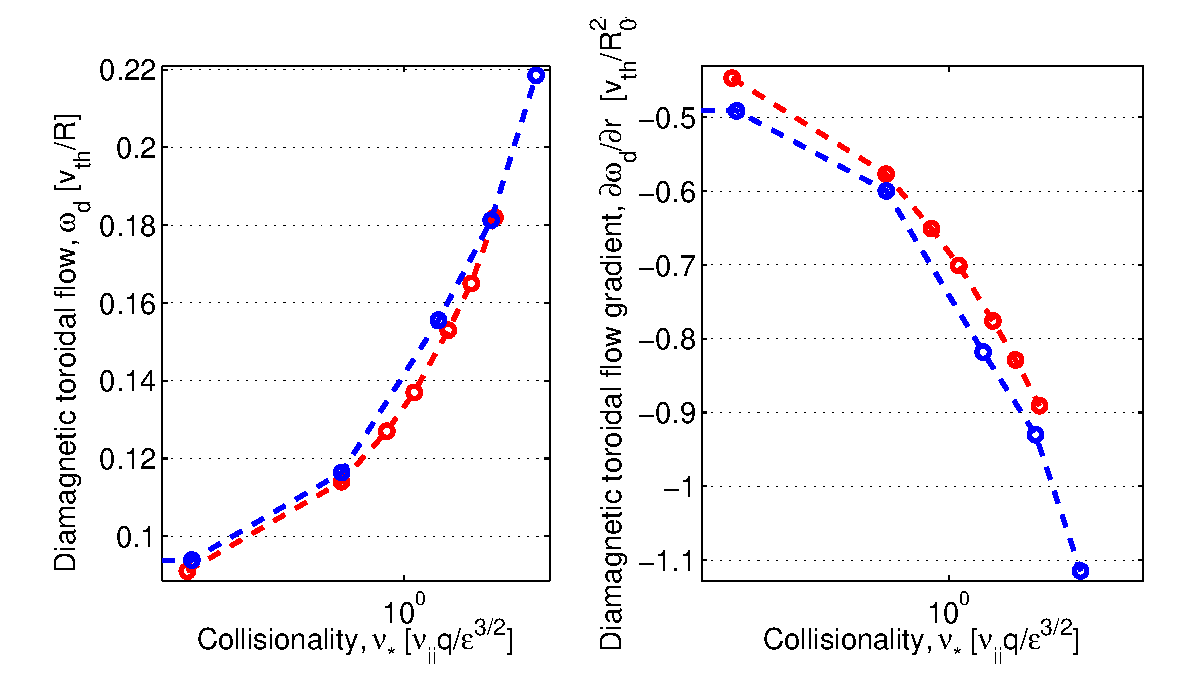
\includegraphics[width=9cm,clip]{Flowscombined.eps}
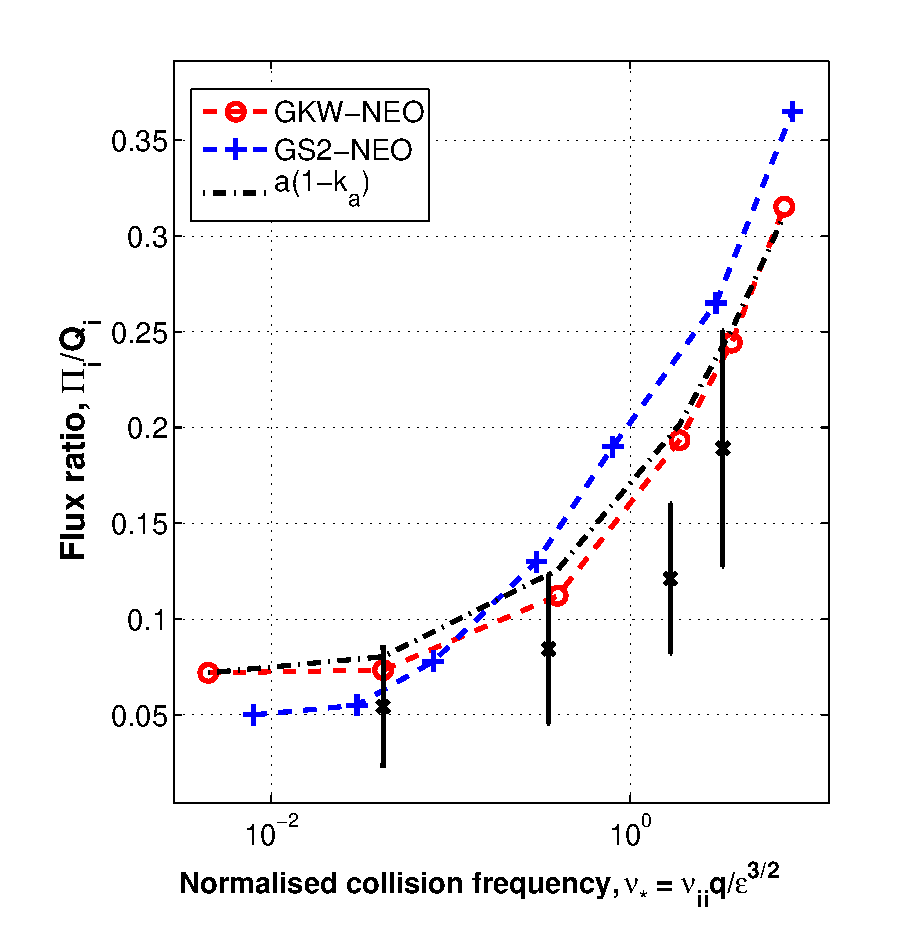
\includegraphics[width=9cm,clip]{GKWGS2QLbenchmark.eps}
\caption{(top) The ratio of the quasi-linear radial flux of toroidal momentum ($\Pi_{i}$) with the radial heat flux ($Q_{i}$) as a function of collisionality for both GKW-NEO (red) and GS2-NEO (blue) at $\rho_{*}=0.089$.  Also plotted (black dashed line) is $a(1-k_{a})$ where a is fitted to the value from GKW-NEO at the zero collisionality limit.  Black crosses represent data from non-linear simulations, the error bars represent the standard deviation of the fluctuations over the statistical steady state part of the simulation.  (bottom) The toroidal diamagnetic frequency, $\omega_{\zeta,d}$ (left) and its radial gradient, $\partial\omega_{\zeta,d}/\partial r$ (right) for runs with GKW-NEO (blue) and GS2-NEO (red) as a function of the normalised collisionality, GS2-NEO data taken from \cite{BarnesParra13} for $\rho_{*}=0.01$. }
\label{neo:gkwgs2comp}
\end{centering}
\end{figure}

Figure~\ref{neo:gkwgs2comp} (left) shows the diamagnetic flow and its gradients as a function of the normalised collision frequency for both GS2-NEO and GKW-NEO for the above parameters, showing good agreement between the two codes.   Figure \ref{neo:gkwgs2comp} shows the turbulent parallel momentum flux ($\Pi_{i}$) normalised to the radial heat flux ($Q_{i}$) for a scan in the collisionality as calculated by GKW-NEO (Red) and GS2-NEO (Blue) for a series of linear simulations at the single toroidal wave number of $k_{\zeta}\rho_{i} =0.4242$. 

\section{Sample input}

A sample NEO input file for the Cyclone base case run, most of the parameters here are ignored as they are read from the input.profile file found in the benchmarks folder in the GKW repository

This uses the code in profile mode and the full Fokker-Plank collision operator.  Most of the parameters are overridden by those in the input profile file.

\begin{verbatim}
PROFILE_MODEL=2
PROFILE_EQUILIBRIUM_MODEL=1
EQUILIBRIUM_MODEL=1
COLLISION_MODEL=4
ROTATION_MODEL=1
N_ENERGY=10
N_XI=19
N_THETA=41
N_RADIAL=5
N_SPECIES=2
Z_1=1
Z_2=-1
MASS_2=  0.00027245
DENS_2=1
RMIN_OVER_A=0.49000000
RMIN_OVER_A_2=0.51000000
RMAJ_OVER_A=3.40730000
KAPPA=  1.28760000
S_KAPPA=  0.01117700
DELTA=  0.07159200
S_DELTA=  0.02895700
SHIFT= -0.10774000
Q=  1.24770000
SHEAR=  0.34412000
OMEGA_ROT=  0.05153600
OMEGA_ROT_DERIV=  0.03058600
RHO_STAR=  0.00776240
DLNNDR_1=  0.0
DLNTDR_1=  0.0
DENS_1=  0.82927000
NU_1=  0.00118530
TEMP_2=  1.17130000
DLNNDR_2=  0.0
DLNTDR_2=  0.0
TEMP_1=1
\end{verbatim}

In the GKW input file the following amendments need to be made to read in the NEO files correctly.

\begin{verbatim}
 &LINEAR_TERM_SWITCHES
 lneo_equil = .true.
 /
 \end{verbatim}
 
 It is possible to apply the neoclassical background to all or a simply a subset of the species in GKW.  Each species in GKW can be pointed to a specific species in NEO.  For example when 

 \begin{verbatim}
&LINEAR_TERM_SWITCHES
 lneo_equil = .true.
 neo_equil_parse_sp_seq = 1,2,3,3
 /
 \end{verbatim} 
 
 is used, for a four species run in GKW for a three species NEO run, then GKW species 3 and 4 use the flow from species 3 in NEO.  This allows the effects of flows on trace species with different parameters to be studied.
